% !TeX spellcheck = en_GB
\documentclass[10pt,oneside,slovak,a4paper]{article}
\usepackage[slovak]{babel}
\usepackage[T1]{fontenc}
\usepackage[IL2]{fontenc} % lepšia sadzba písmena Ľ než v T1
\usepackage[utf8]{inputenc}
\usepackage{graphicx}
\usepackage{url} % príkaz \url na formátovanie URL
\usepackage{hyperref} % odkazy v texte budú aktívne (pri niektorých triedach dokumentov spôsobuje posun textu)
\usepackage{cite}
%\usepackage{times}
\pagestyle{headings}
\usepackage{graphics}
\usepackage{pgfplots}
\pgfplotsset{compat=1.16}


\title{5G a umelá inteligencia vo vzdelávaný\thanks{Semestrálny projekt v predmete Metódy inžinierskej práce, ak. rok 2020/21, vedenie:}} 

\author{Juraj Ševčík\\[2pt]
	{\small Slovenská technická univerzita v Bratislave}\\
	{\small Fakulta informatiky a informačných technológií}\\
	{\small \texttt{xsevcik@stuba.sk}}
}

\date{\small 20. oktober 2020}


\begin{document}

\maketitle

\begin{abstract}


\end{abstract}
V súčasnosti  keď je elektronické vzdelávanie dôležitejšie ako kedykoľvek predtým nadišli vhodný čas zamerať sa na to kam až sa dá z dnešnou technológiou posunúť a ako ju najvhodnejšie implementovať. Z postupným nástupom 5G a znižovania latencie medzi používateľom a serverom na 1-3 ms sa otvára celí nový smer implementácie umelej inteligencia z možnosťou prispôsobiť učebné postupy a metódy v reálnom čase na základe špecifických potrieb a pokrokov študenta.  5G je taktiež ideálnym prostriedkom pre študentov so špeciálnymi potrebami ci pre učiteľov aby dostali lepšiu a rýchlejšiu odozvou od študentov.
Umelá inteligencia je vďaka už spomenutej nízkej latencii schopná nie len prispôsobovať študijný plán ale ho aj v reálnom čase analyzovať  a vyhodnocovať v pre nás zatiaľ nemysliteľných smeroch. Preto je potrebné sa sústrediť na tvorbu vzdelávacích platforiem ktoré integrujú 5G a umelú inteligenciu.

\newpage
\section{Úvod}



5G je môžemem adaptovať aj na špecifické odbory kde majú velké využitie ako napríklad pre študentov vysoých škôl ktorý vdaka vačšiemu množstvu prenášaných dát budú mať možnosť vyrtuálne preštudovať pamiatok bežne neprístupních návštevníkom čím by umožnily študentom vyrtuálne navštiviť katakombi pod piramídami v Gýze čí Lascauckú jaskinu vo Francúzku. Tiež pre študenťov chémie ktorý môžu vykonávať experimenty vo vyrtálnom priestore ktorý by bol napojený na hlavný počítač ktorý by zabezpečoval výkon ktorý nedokážu poskitnúť "menšie" zariadenia. 

Nové technologie by tiež priniesly zmenu do samotneho systému vzdelavania kde by upustilo od zastaraneho memorovania a pristupilo by sa k získavaniu vedomostí pomocov experimentov a skumania z minimálnim zásahom učitela.\cite{Opincariu2019EDUCATIONIT}


%Umelá inteligencia je vďaka už spomenutej nízkej latencii schopná nie len prispôsobovať študijný plán ale ho aj v reálnom čase analyzovať  a vyhodnocovať v pre nás zatiaľ nemysliteľných smeroch. Preto je potrebné sa sústrediť na tvorbu vzdelávacích platforiem ktoré integrujú 5G a umelú inteligenciu.
\begin{itemize}
\item Podla oxfordskeho slovníka e-vzdelavanie je systém vzdelávania ktorý využíva elektronické médiá zvičajne cez internne. 

Pod e-vzdelávaním teda rozumieme akékolvek zvdélávanie pomocou internetu či íných elektronických zariadení od mobilných telefónov či tabletov až po sústavy na vyrtuálnu realitu či najrôznejšie softverové časti ako webstaránky či vyučovacie softvery. Všetky tieto technologie prenášajú možnosť vzdelávať bližšie ako dedikolvek predtím a umožnujú rpístum k najrôznejším sposobom vzdelávanie v skoro všetkých oblastiach.

\item 
5G je piata generácia mobilnej komunikácie začala sa objavovať od roku 2019 ako nástupca 4G táto efektivna technologia podporuje viac zariadený a vačšiu rýchlosť čím umožnuje používať viac zariadený na opercie s vyžšov spotrebou dát a menšou latenciou, taktiež to otvorý celé nové spektrum technológií ako autonómne autá, smart city, vyrtualna realita či IoT ktoré sa stane spolahlivejším, rýchlejším a užitočnejším.

\item 
Umelá inteligencia, alebo tiež artificial intelligence(AI), podla Housmana (2018): ''AI je schopná dvoch vecí: automatizovanie repetitívnich úloch predpovedaním výstupu na základe dát ktoré boly cložene človekom a vylepšovať ludské rozhodnutia zadávaním problemov do algoritmov vyvinutých človekom. ''

Umelá inteligenia nieje inteligencia v biologickom slovazmysle, je to neorganický system napodobnujúci procesy myslenia a vyvodzovania výsledkov a to všetko na základe vtupov a algotitmov do nej vložených.  


%John McCarthy a Marvin Minsky : "Umelá inteligencia je akákolvek aktivita vzkonaná strojom o ktorej sa dá povedať že keby su vykonával človek musel by použit inteligenciu." 

\end{itemize}

\section{Možnosti využitia} 
Mnohé programy implementuju AI, a nachádza si miesto od smartfónov cez autonomne autá, inteligentne domácnosti ......a v neposlednom rade aj v školstve zatial prevažne na univerzitách ale postupne prichádza aj do nižších ročnikov.

V budúcnosti by sa mala stať bežnov a základnov častov vzdelávania kde žiakom poskitne možnosti dnes už dôverne známich osobních(personalizovaných) nastavený. Nastavený ktoré vidíme v smartfonooch či aplikáciách a umožnujú nám najrôznejšie prispôsobenia pre naše pohodlie a maximálne využitie daného nástroja. Osobné nastavenie by sa malo stať novým štandardom a ponúkať študentom personalizované vyučovacie plány na základe ich znalostí a schopností.

\subsection{Vyučovacie aplikacie}

Aplikacie zo začlenennov umelov inteligenciou získavajú dáta a v reálnom čase ich spracovávaju a vzhodnocujú či prispúôsobujú aby maximalizovaly svoj dopad a poskitly najvodnejsie materialy na základe predošlích skusenosťí, zanlosťí študenta a jeho osobytníc schopností.

Elektronizácia poskytne viac času pre učitelov aby sa venovaly žiakom ktorý to potrebujú alebo aby riešily problemy ktoré vyžadujú ichh pozornosť.  

\begin{figure}[h!]
	%\centering
	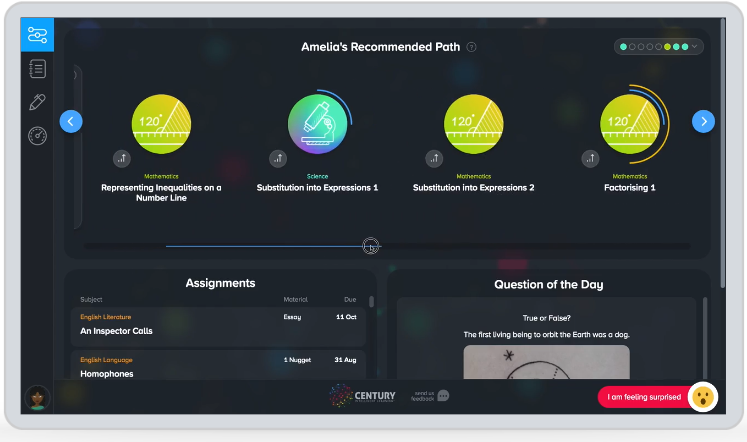
\includegraphics[width=0.7\linewidth]{obrazky/artificial-intelligence-applications-edtech-century-tech}
	\caption{}
	\label{fig:artificial-intelligence-applications-edtech-century-tech}


\subsection{QUERIUM}
\ref{khanacademy}
Queriumje aplikacia obsahujúca umelú inteligenciu ktorú používa na prispôsobenie obsahua kontrolu postupu pri riešený metematických problémov. V aplikácii žiaci počítajú príklady krok po kroku a dostávajú okamžitú spätnú väzbu, toto riešeni dáva učitelom viac času zamerať sa na jednotlivých študentov. Aplikácia tektiež poskytuje spätnú väzbu na postup študentov kde sa učitelia dozvedia v ktorých krokokch a mali špecialne študenti problém a ktoré časti učiva je potrebné špeciálne zopakovať takže učitel nemusí prechádzať cez celé učivo znova a môže sa zamerať len na podstatné časti čím zisakjú viac časuna zatial neprebrané učivo.

Súčastov Queria sú aj vidéa o ku témam, rýchli test ktorý preverí ake vedomasti a identifikuje slabé a silné stránky aby na základe toho prispôsobil osnovy.



\subparagraph{vysledky:}
V roku 2014 sa 11 študentov zúčastnilo testu pred a po používaný aplikácie, vyše 90 \% študentov si zlepšilo skóre v priemere o 10 bodov a až na jedneho študenta aplikácia šetkým pomohla. \ref{tabulka} \ref{querium_report}

\end{figure}
\label{tabulka}
%graf querium 
\pgfplotstableread[row sep=\\,col sep=&]{
	interval & pred & po  \\
	1        & 315  & 327 \\
	2    	 & 310  & 332 \\
	3    	 & 322  & 337 \\
	4    	 & 340  & 340 \\
	5    	 & 339  & 342 \\
	6    	 & 335  & 342 \\
	7    	 & 342  & 347 \\
	8    	 & 338  & 350 \\
	9    	 & 338  & 351 \\
	10       & 345  & 351 \\
	11       & 342  & 352 \\
	
	
}\mydata


\begin{tikzpicture}
\begin{axis}[
ybar,
symbolic x coords={1,2,3,4,5,6,7,8,9,10,11},
]
\addplot table[x=interval,y=pred]{\mydata};
\addplot table[x=interval,y=po]{\mydata};
\end{axis}

\end{tikzpicture}


\subparagraph{Vyučovacie aplikacie}

Rozšírena realita  (využitím umelej inteligencie na spravne umiestnenie objektov) obohacuje biologiu, geografiu ,fyziku pre deti nyžších rčníkov....Londín()
\cite{AI}
\subsection{ine študijne aplikacie}
Umelá ointeligancia napojená pomocov vysokorýchlostného pripojenia je schopná využívať data mining algoritmus v reálnom čase a tým odokrívať nám nepoznané prepojenia a suvýslosti je schopný predefinovať spôsob akým dnes vnímame zdelanie ktoré je založeneé na metódach ktoré už boly vyvinuté už pred rokmy a nebralin  do úvahy technologické možnosti budúcnosti.


Dalšie aplikacie na pomoc študentom ako napríklad Nuance, na prepisovanie dovoého textu na poznamky alebo ine na prepisanie textu z tofografie na textový súbor ....matematicke aplikacie ...


%\section{Nevýhody}

%\subsection{v čom AI zliháva }

\section{psychologický aspekt evzdelavanie }
Evzdelávanie má svoje výhody aj nevýhody môže poskitnú študentom viac času kedže nemusia cestovať a hodín sa zučstnovať fyzicky ale na druhej strane môže tím utrpieť aspekt socializácie, tento fakt je dôležitý hlavne v súčastnej dobe pandémmie ked je celospoločenská socializácia značne obmedzená, ale je nutné podotknuť že za iných okolností by práve aspekt e vzdelavania mohol pomôcť k lepšej socialnej zrelosťi žiakov pretože to je oblasť kde by sa presunula hlavná hlavná pozornosť mimo elektronických systémov a verím že táto časť by stále prebiehala ofline 
>nižšia socializácia 
>"neosobnejší" pristup ale možnost adaptovat študijni plan 
>vôčšia pozornost pre jednotlivých študentov ....

\section{ako e vzdelavanie ovplvnilo školstvo}
Evzdelávanie postupne už dlhšie preniká do školstva kde pôsobý pozitívny pokrok tým že poiskitlo prístup k mnohým materiálom napríklad v súčstnosti je velké množstvo videý a vzučovacích programov dostupných online čo otvorilo možnosťy keď je odborný výklad vzdialený len na pár klikov. 

Softvéry ktoré su schopné symulovať či tvorit ....\cite{10.1145/3399971.3399984}


- dalo učitelom viac času na jednotlivých studentov 
-nove možnosti vzdelavania 

\section{kedy a ako môžeme očakavat 5G a AI v triedach}



\bibliography{bibligraficky_subor}

\bibliographystyle{ieeetr}
%\begin{thebibliography}{9}
	
\label{khanacademy} 
\texttt{https://www.khanacademy.org/}
\\
\label{AI} 
\texttt{https://www.nttdata.com/mm/en/digital/ai/2018/september/what-is-ai}
\date{22.11.2020}
\\
\label{querium_report}
\texttt{https://querium.com/wp-content/uploads/Querium-TSI-Math-Prep-Spring-2014-Beta-Test-Preliminary-Results.pdf}

	
	
%\end{thebibliography}

\end{document}

